\documentclass[english,serif,mathserif,usenames,dvipsnames]{beamer}
\usetheme[informal]{gc3}

\usepackage[T1]{fontenc}
\usepackage[utf8]{inputenc}
\usepackage{babel}

%% This is optional: it adds a few commands and environment we
%% regularly use in our slide sets
\usepackage{gc3}

\begin{document}

\title[ElastiCluster]{ElastiCluster} \subtitle{\bfseries Automated provisioning
  \\ of computational clusters in the cloud} \author{%
  Riccardo Murri \texttt{<riccardo.murri@gmail.com>} \\
  \smaller\itshape (with contributions from Antonio Messina, Nicolas Bär, \\
  Sergio Maffioletti, and Sigve Haug) }
\date{HEPiX Spring 2017}

%% Makes the title slide
\maketitle


\begin{frame}
  \frametitle{What is ElastiCluster}

  ElastiCluster provides a \textbf{command line tool} to \textbf{create, set up
    and scale} computing clusters hosted on IaaS cloud infrastructures.

  \+
  Main function is to get a compute cluster up and running with a single command.

  \+
  Additional commands can scale the cluster up and down.
\end{frame}


\begin{frame}[fragile]
  \frametitle{Example: SLURM cluster}

    Cluster definition is done in a INI-format text file.

    \lstdefinelanguage{ini}{%
      morekeywords={%
        cloud,
        login,
        setup,
        frontend\_nodes,
        compute\_nodes,
        ssh\_to,
        security\_group,
        image\_id,
        flavor,
        frontend\_groups,
        compute\_groups,
        provider,
        auth\_url,
        username,
        password,
        project\_name,
        image\_user,
        image\_user\_sudo,
        image\_sudo,
        user\_key\_name,
        user\_key\_private,
        user\_key\_public,
      },
      sensitive=true,
      morecomment=[s]{[}{]},
    }%
    \lstset{%
      language=ini,
      escapechar=@,
      basicstyle=\footnotesize\ttfamily\color{gray},
      commentstyle=\bfseries\color{gray},
      keywordstyle=\bfseries\color{black},
    }%
    \begin{columns}
      \begin{column}{0.5\linewidth}
        \footnotesize
\begin{lstlisting}
[cluster/slurm]
cloud=openstack
login=ubuntu
setup=slurm
frontend_nodes=1
compute_nodes=4
ssh_to=frontend
security_group=default
image_id=...
flavor=4cpu-16ram-hpc

[setup/slurm]
frontend_groups=slurm_master
compute_groups=slurm_worker
\end{lstlisting}
      \end{column}
      \begin{column}{0.5\linewidth}
        \footnotesize
\begin{lstlisting}
[cloud/openstack]
provider=openstack
auth_url=http://...
username=***
password=***
project_name=***

[login/ubuntu]
image_user=ubuntu
image_user_sudo=root
image_sudo=yes
user_key_name=elasticluster
user_key_private=
    ~/.ssh/id_rsa
user_key_public=
    ~/.ssh/id_rsa.pub
\end{lstlisting}
      \end{column}
    \end{columns}

\end{frame}


\begin{frame}
  \frametitle{ElastiCluster demo}

  \begin{enumerate}
  \item Create 4 virtual machines on an OpenStack cloud
  \item Install and configure a SLURM cluster on them
  \item Connect to the cluster
  \item Run an example
  \item Add 1 more node to the cluster
  \item Destroy the cluster when done
  \end{enumerate}

  \+
  \begin{center}
    \Large
    \href{http://www.youtube.com/watch?v=DDm6-QEnNsU}{\textbf{show time!}}
  \end{center}
\end{frame}


\begin{frame}
  \frametitle{ElastiCluster features (1)}

  \begin{columns}
    \begin{column}{0.5\linewidth}
      \emph{Computational clusters supported:}
      \begin{itemize}
      \item Batch-queuing systems:
        \begin{itemize}
        \item SLURM
        \item GridEngine
        \item Torque+MAUI
        \item {\color{gray} HTCondor}
        \end{itemize}
      \item Spark / Hadoop 2.x
      \item {\color{gray} Mesos + Marathon}
      \end{itemize}
    \end{column}
    \begin{column}{0.5\linewidth}
      \emph{Distributed storage:}
      \begin{itemize}
      \item GlusterFS
      \item HDFS
      \item OrangeFS/PVFS
      \item {\color{gray} Ceph}
      \end{itemize}

      \+
      \emph{Optional add-ons:}
      \begin{itemize}
      \item Ganglia
      \item JupyterHub
      \item EasyBuild
      \end{itemize}
    \end{column}
  \end{columns}

  \+
  \begin{center}
    \footnotesize\em
    ({\color{gray} Grayed out} items have not been
    tested in a while\ldots)
  \end{center}
\end{frame}


\begin{frame}
  \frametitle{ElastiCluster features (2)}

  Run on multiple clouds:
  \begin{itemize}
  \item Amazon EC2
  \item Google Compute Engine
  \item OpenStack
  \end{itemize}

  \+
  Supports several distros as base OS:
  \begin{itemize}
  \item Debian 7.x (\emph{wheezy)}, 8.x \emph{(jessie)}
  \item Ubuntu 14.04 \emph{(trusty)}, 16.04 \emph{(xenial)}
  \item CentOS 6.x, 7.x
  \item Scientific Linux 6.x
  \end{itemize}
\end{frame}


\section{Architecture and implementation}
\begin{frame}
  \frametitle{How does ElastiCluster work?}

  \begin{enumerate}
  \item Create virtual machines in a cloud
    \begin{itemize}
    \item done by Python code in ElastiCluster
    \end{itemize}

  \item Install and configure a pre-defined set of software
    \begin{itemize}
    \item delegated to \href{http://www.ansible.com}{Ansible}
    \end{itemize}
  \end{enumerate}
\end{frame}


\begin{frame}
  \frametitle{Software setup (1)}

  ElastiCluster leverages \href{http://www.ansible.com}{Ansible} \\
  to deploy and configure software:
  \begin{itemize}
  \item ``playbooks'' are list of idempotent tasks
    \begin{itemize}
    \item playbooks can be re-run many times over
    \item changes are \textit{exactly reproducible}
    \end{itemize}

  \item everything is on the client machine
    \begin{itemize}
    \item no agent or bootstrap needed on cloud VMs
    \item all configuration / playbooks hosted in a single place
    \end{itemize}

  \item works on base OS images
    \begin{itemize}
    \item independent from the cloud infrastructure
    \end{itemize}
  \end{itemize}
\end{frame}


\begin{frame}
  \frametitle{Software setup (2)}
  In a sense, ElastiCluster is just a large collection of Ansible playbooks.

  \+ But there is nothing special about these playbooks: \textbf{any Ansible
    playbook can be applied by ElastiCluster}

  \+ So, you can \emph{replace} ElastiCluster's playbooks, \\
  or \emph{add} you own ones.
\end{frame}


\begin{frame}
  \frametitle{Issues}
  Setup time grows \emph{linearly} \\ with the number of cluster nodes.

  \+
  Overcoming this seems to require a major change \\ in how cluster setup is
  executed.

  \+
  Ongoing discussion at: \url{https://github.com/elasticluster/elasticluster/issues/365}
\end{frame}


\begin{frame}
  \frametitle{Performance tip \#1}

  To speed up setup, we need to reduce the amount of work that
  Ansible has to do:
  \begin{enumerate}
  \item create a prototype cluster;
  \item make snapshots of each node type;
  \item \textbf{create clusters using the snapshots}
    \\ instead of the base OS image.
  \end{enumerate}

\end{frame}


\begin{frame}
  \frametitle{Performance tip \#2}

  Ansible can run many playbooks in parallel.

  \+
  But the default degree of parallelism is very conservative.

  \+
  \textbf{Increase the number of parallel connections!} \\
  A 1Gb/s network and a multicore CPU can easily accomodate a few 100's parallel
  SSH connections.
\end{frame}


\begin{frame}
  \frametitle{Performance tip \#3}

  Setup time grows with the number of \emph{nodes}.

  \+
  If you only care about CPU core count, \\
  \textbf{use larger VM instance flavors}.
\end{frame}


\section{Experiences}
\begin{frame}
  \frametitle{Typical use cases}
  \begin{itemize}
  \item \textbf{On demand provisioning} \\ of computational cluster
  \item Clusters/servers for \textbf{Teaching}
  \item \textbf{Testing} new software or configurations
  \item \textbf{Scaling} a permanent computing infrastructure
  \end{itemize}
\end{frame}


\begin{frame}
  \frametitle{On-demand provisioning of compute clusters}

  \href{https://cloud.google.com/genomics/}{Google Genomics} provides
  instructions to its users to spin up ephemeral GridEngine clusters.

  \+
  \uncover<2>{%
    \smaller
    \begin{quotation}
      ``The instructions presented here are guidelines that have been used to
      create clusters up to 100 nodes. However when preemption rates are high,
      Elasticluster’s re-provisioning of clusters (via Ansible) often converges
      too slowly due to repeated failures.

      For best success with the instructions here, it is recommended to keep
      cluster sizes to 20 compute nodes or fewer. For larger clusters, use
      regular (non-preemptible) virtual machines.''
    \end{quotation}
  }%

  \+
  \begin{references}
    \tiny
    \begin{itemize}
    \item
      \url{http://googlegenomics.readthedocs.io/en/latest/use_cases/setup_gridengine_cluster_on_compute_engine/index.html}
    \item
      \url{http://googlegenomics.readthedocs.io/en/latest/use_cases/setup_gridengine_cluster_on_compute_engine/preemptible_vms.html}
    \end{itemize}

  \end{references}
\end{frame}


\begin{frame}
  \frametitle{Clusters for teaching}
  \emph{At UZH:} JupyterHub+Spark clusters \\ for teaching courses
  (e.g., data science) \\ or for short-lived events (e.g., workshops).

  \+
  \emph{At UniBas:} make tiny ``replica'' clusters \\ to teach new users.

  \+
  \textbf{Key ingredient is the ability to apply custom Ansible playbooks on
    top}
  of the standard ones, \\ to make per-event customizations.
\end{frame}


\begin{frame}
  \frametitle{Scaling permanent clusters}
  \emph{At UniBE:} additional WLCG cluster for ATLAS analysis hosted on
  \href{http://engines.switch.ch/}{SWITCHengines}

  \+
  \smaller
  \alt<2>{%
    \begin{quotation}
      ``A 304 virtual CPU core Slurm cluster was then started with one command on
      the command line. This process took about one hour. A few post-launch steps
      were needed before the cluster was production ready. However, a skilled
      system administrator can setup a 1000 core elastic Slurm cluster on the
      SWITCHengines within half a day. {\bfseries As a result the cluster becomes a transient
      or non-critical component. In case of failure one can just start a new one,
      within the time it would take to get a hard disk exchanged.}''
    \end{quotation}
  }{%
    \begin{center}
      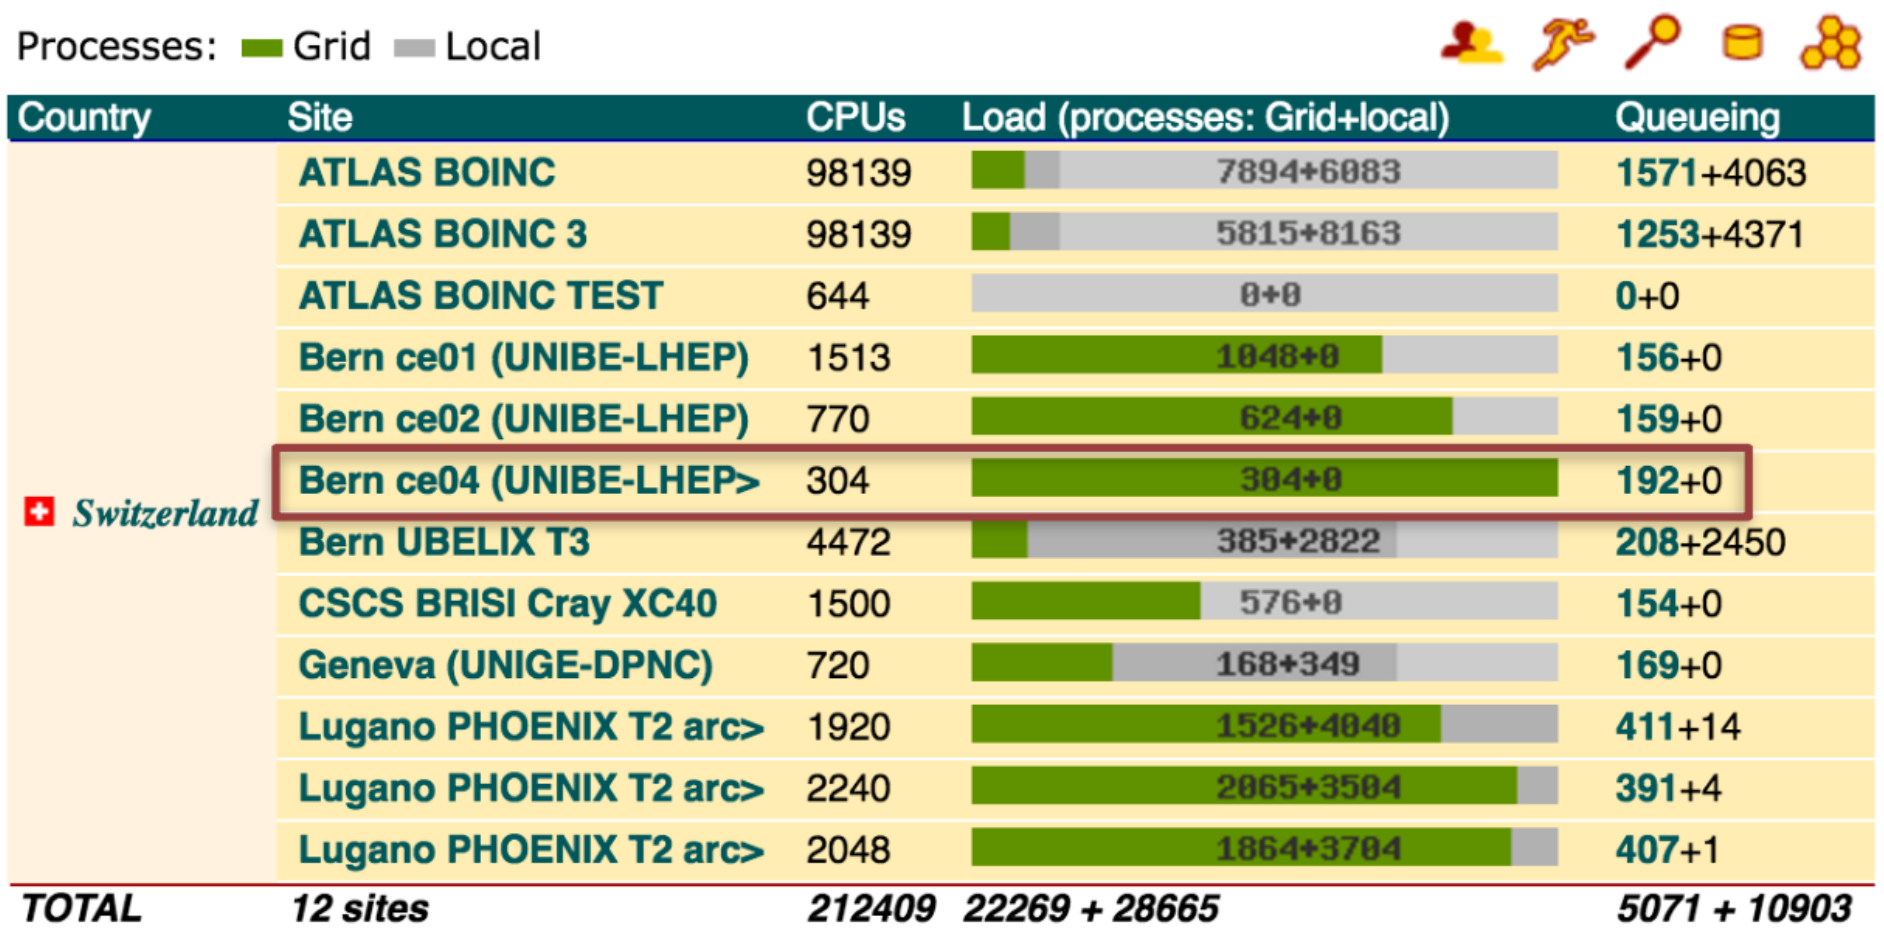
\includegraphics[width=0.80\linewidth]{arc-monitor-unibe.png}
    \end{center}
  }%

  \centering
  \begin{references}
    \tiny
    S.~Haug and G.~F.~Sciacca,
    ``ATLAS computing on Swiss Cloud SWITCHengines'',
    CHEP 2016
  \end{references}
\end{frame}


\section{The End}
\begin{frame}[fragile]
  \frametitle{Any questions?}

  \begin{center}

  ElastiCluster source code:
  \url{http://github.com/gc3-uzh-ch/elasticluster}

  \+
  ElastiCluster documentation:
  \url{https://elasticluster.readthedocs.org}

  \+
  Mailing-list: \\
  \url{elasticluster@googlegroups.com}

  \+
  Chat / IRC channel: \\
  \url{http://gitter.im/elasticluster/chat}
  \end{center}
\end{frame}


\begin{frame}
  \frametitle{Credits}

  The initial ElastiCluster dev team:
  \begin{itemize}
  \item Antonio Messina \texttt{<antonio.s.messina@gmail.com>}
  \item Nicolas B\"ar \texttt{<nicolas.baer@gmail.com>}
  \end{itemize}



  \ldots and the many users at UZH who, wittingly or not, have used
  ElastiCluster, reported bugs, and suggested improvements.

\end{frame}
\end{document}

%%% Local Variables:
%%% mode: latex
%%% TeX-master: t
%%% End:
